
\chapter{Encoding BAN logic}
\label{chap:BAN}

Burroughs-Abadi-Needham (BAN) logic is a logic of authentication-protocols. It's of interest in Jape chiefly because it is a logic in which the rules don't fit into a tidy introduction / elimination structure, so it takes some ingenuity to design menus and double-clicking mechanisms to suit. Also, conjectures seem naturally to require long lists of assumptions, which makes it possible to demonstrate Jape's mechanism for folding long association lists. And its use of tuples demonstrates some new ways in which Jape can deal with families of rules.

\section{Syntax}

The syntax of the logic is very simple, although it includes a number of novel operators, most of which are in Unicode (though I never found a glyph for |$\sim$). I had to linearise some of the notation: for example, $A\overset{K}{<->}B$ ($A$ and $B$ share private key $K$) became $( A,B)<->K$ and $\{ X\}_{K}$ ($X$ encrypted by $K$) is now $\{X\}K$. Otherwise, I hope, I faithfully described the syntax, even if I had to guess at the syntactic hierarchy of operators.

In \texttt{examples/BAN} there are two versions of the encoding: \texttt{BAN.jt} for those who have a appropriate Unicode font available, and \texttt{BAN\_ASCII.jt} for those who are prepared to put up with multi-character approximations. They are intended to be identical up to representations of the operators. The examples in this chapter are taken from the ASCII version, because even I don't have a proper Unicode font yet.

From \texttt{BAN\_ASCII\_syntax.jt}:
\begin{japeish}
CLASS VARIABLE x k \\
CLASS FORMULA W X Y Z \\
CLASS CONSTANT P Q R K N T \\
CONSTANT A B S \\
 \\
SUBSTFIX    700 \\
JUXTFIX     600 \\
PREFIX      500     \# \\
POSTFIX     500     ⁻¹ \\
INFIX       300L    ⇌  ↦ ↔ \\
INFIX       200R    |$\sim$ \\
INFIX       150R    |⇒ \\
LEFTFIX     110 ∀ . \\
INFIX       100R    |≡ \\
INFIX       50L     <| \\
 \\
OUTFIX {  } \\
OUTFIX <  > \\
 \\
BIND x SCOPE P IN ∀x . P \\
SEQUENT IS BAG ⊢ FORMULA \\
INITIALISE autoAdditiveLeft true
\end{japeish}

\section{Rules}

The rules of the logic are described in [``A Logic of Authentication'', Burrows, Abadi, Needham] which is available on the Web from Mart\'{\i}n Abadi's home page, or in paper form as (Proceedings of the Royal Society, Series A, 426, 1871 (December 1989), 233-271). Two of the rules have a `$\mathrm{from}\,R$' side-condition which I didn't understand so haven't implemented. The rules are given natural-deduction style, without mentioning a context of hypotheses, but they don't have an introduction / elimination structure so far as I can see:
\begin{ruletab}{|l|l|l|l|}
\hline
% ROW 1
$\infer	{P \believes Q{\oncesaid}X}
		{P \believes Q\overset{K}{<->}P & P \sees \{X\}_{K}}$ 
&
$\infer	{P \believes Q{\oncesaid}X}
		{P \believes \,\overset{K}{|->}Q & P \sees \{ X\}_{K^{-1}}}$
&
\multicolumn{2}{|l|}{
$\infer {P \believes Q{\oncesaid}X}
		{P \believes Q \overset{Y}{\rightleftharpoons}P & 
		 P \sees \left\langle X\right\rangle_{Y}}$}
\\
\hline
% ROW 2
\multicolumn{2}{|l|}{
$\infer	{P \believes Q \believes X}
		{P \believes \#X & P \believes Q{\oncesaid}X}$}
&
\multicolumn{2}{|l|}{
$\infer	{P \believes X}
		{P \believes Q \hasjurisdictionover X & P \believes Q \believes X}$}
\\
\hline
% ROW 3
$\infer	{P \believes (X,Y) }
		{P \believes X & P \believes Y}$
&
$\infer	{P \believes X}
		{P \believes (X,Y) }$
&
$\infer	{P \believes Q \believes X}
		{P \believes Q \believes (X,Y) }$
&
$\infer	{P \believes Q \oncesaid X}
		{P \believes Q \oncesaid (X,Y) }$
\\
\hline
% ROW 4
$\infer	{P \sees X}
		{P \sees (X,Y) }$
&
$\infer	{P \sees X}
		{P \sees \left\langle X\right\rangle _{Y} } $
&
&
\\
\hline
% ROW 5
$\infer	{P \sees X}
		{P \sees Q\overset{K}{<->} P & P \sees \{ X\}_{K}} $
&
$\infer	{P \sees X}
		{P \believes \,\overset{K}{|->}P & P \sees \{ X\}_{K}} $
&
\multicolumn{2}{|l|}{
$\infer	{P \sees X}
		{P \believes \,\overset{K}{|->}Q & P \sees \{ X\}_{K^{-1}}} $}
\\
\hline
% ROW 6
$\infer	{P \believes \#(X,Y) }
		{P \believes \#X}$
&
&
&
\\
\hline
% ROW 7
$\infer	{P \believes R' \overset{K}{<->} R}
		{P \believes R\overset{K}{<->} R' } $
&
$\infer	{P \believes Q \believes R' \overset{K}{<->} R}
		{P \believes Q \believes R\overset{K}{<->} R' } $
&
$\infer	{P \believes R' \overset{X}{\rightleftharpoons} R}
		{P \believes R\overset{X}{\rightleftharpoons} R' } $
&
$\infer	{P \believes Q \believes R' \overset{X}{\rightleftharpoons} R}
		{P \believes Q \believes R\overset{X}{\rightleftharpoons} R' } $
\\
\hline
% ROW 8
\multicolumn{4}{|l|}{
$\infer	{P \believes Q \hasjurisdictionover 
		 X\left[ v_{1} ...v_{n} \backslash Y_{1} ...Y_{n} \right] }
		{P \believes @*v_{1}, \dots , v_{n} .(Q\hasjurisdictionover X) } $}
\\
\hline
\end{ruletab}


The rules which don't deal with tuples are straightforwardly encoded:
\begin{japeish}
RULE "P|≡(Q,P)↔K, P<|\{X\}K ⇒ P|≡Q|$\sim$X" IS \\
\tab FROM P|≡(Q,P)↔K AND P<|\{X\}K INFER P|≡Q|$\sim$X\\
RULE "P|≡Q↦K, P<|\{X\}K⁻¹ ⇒ P|≡Q|$\sim$X" IS \\
\tab FROM P|≡Q↦K AND P<|\{X\}K⁻¹ INFER P|≡Q|$\sim$X\\
RULE "P|≡(P,Q)⇌Y, P<|<X>Y ⇒ P|≡Q|$\sim$X" IS \\
\tab FROM P|≡(P,Q)⇌Y AND P<|<X>Y INFER P|≡Q|$\sim$X\\
RULE "P|≡\#X, P|≡Q|$\sim$X ⇒ P|≡Q|≡X" IS \\
\tab FROM P|≡\#X AND P|≡Q|$\sim$X INFER P|≡Q|≡X\\
RULE "P|≡Q|⇒X, P|≡Q|≡X ⇒ P|≡X" IS \\
\tab FROM P|≡Q|⇒X AND P|≡Q|≡X INFER P|≡X
\end{japeish}
\begin{japeish}
RULE "P<|<X>Y ⇒ P<|X" IS \\
\tab FROM P<|<X>Y INFER P<|X\\
RULE "P|≡(P,Q)↔K, P<|\{X\}K ⇒ P<|X" IS \\
\tab FROM P|≡(P,Q)↔K AND P<|\{X\}K INFER P<|X\\
RULE "P|≡P↦K, P<|\{X\}K ⇒ P<|X" IS \\
\tab FROM P|≡P↦K AND P<|\{X\}K INFER P<|X\\
RULE "P|≡Q↦ K, P<|\{X\}K⁻¹ ⇒ P<|X" IS \\
\tab FROM P|≡Q↦ K AND P<|\{X\}K⁻¹ INFER P<|X
\end{japeish}
\begin{japeish}
RULE "P|≡(R,R')↔K ⇒ P|≡(R',R)↔K" IS \\
\tab FROM P|≡(R,R')↔K INFER P|≡(R',R)↔K\\
RULE "P|≡Q|≡(R,R')↔K ⇒ P|≡Q|≡(R',R)↔K" IS \\
\tab FROM P|≡Q|≡(R,R')↔K INFER P|≡Q|≡(R',R)↔K\\
RULE "P|≡(R,R')⇌K ⇒ P|≡(R',R)⇌K" IS \\
\tab FROM P|≡(R,R')⇌K INFER P|≡(R',R)⇌K\\
RULE "P|≡Q|≡(R,R')⇌K ⇒ P|≡Q|≡(R',R)⇌K" IS \\
\tab FROM P|≡Q|≡(R,R')⇌K INFER P|≡Q|≡(R',R)⇌K\\
\end{japeish}
\begin{japeish}
RULE "P|≡∀x.X(x) ⇒ P|≡X(Y)"(Y,ABSTRACTION X) IS \\
\tab FROM P|≡∀x.X(x) INFER P|≡X(Y)
\end{japeish}

I had to include hyp so that the context can be used. Cut and left-weakening are, I believe, assumed by the authors:
\begin{japeish}
RULE hyp IS INFER X ⊦ X\\
RULE cut(X) IS FROM X AND X ⊦ Y INFER Y\\
RULE weaken(X) IS FROM Y INFER X ⊦ Y\\
\\
IDENTITY hyp\\
CUT cut\\
WEAKEN weaken
\end{japeish}

\section{Putting rules into menus}

Organising the rules into menus isn't trivial. I've included a menu for each operator and put each rule into all the menus which seem relevant to it: for example, \texttt{"P|≡(Q,P)↔K, P<|{X}K ⇒ P|≡Q|$\sim$X"} is in the menus for $<->$, $\sees$ and $\believes$. Only hyp and the rule dealing with ∀ are in a menu labelled `Logic'.

I implemented forward reasoning in the style of \chapref{ItL}; for example \texttt{"P|≡(Q,P)↔K, [P<|{X}K] ⇒ P|≡Q|$\sim$X"} is included in the $<->$ menu as
\begin{japeish}
ENTRY "P|≡(Q,P)↔K, [P<|{X}K] ⇒ P|≡Q|$\sim$X" IS \\
\tab ForwardOrBackward ForwardCut 0 "P|≡(Q,P)↔K, P<|{X}K ⇒ P|≡Q|$\sim$X"
\end{japeish}
and in the $\triangleleft$ menu as
\begin{japeish}
ENTRY "P<|{X}K, [P|≡(Q,P)↔K] ⇒ P|≡Q|$\sim$X" IS \\
\tab ForwardOrBackward ForwardCut 1 "P|≡(Q,P)↔K, P<|{X}K ⇒ P|≡Q|$\sim$X"
\end{japeish}

The square-bracketed antecedent in the menu entry is the one that \emph{isn't} focussed upon in that step. The whole gory details are in the file \texttt{BAN\_ASCII\_menus.j}. I may not have included the rules in enough menus or enough times (for example, I probably ought to have \texttt{"P<|{X}K, [P|≡(Q,P)↔K] ⇒ P|≡Q|$\sim$X"} in the |$\sim$ menu twice, focussing once on each antecedent). I haven't had enough feedback to know if I got this bit of user interaction right.

\section{Dealing with tuples}

I generalised some of the BAN rules: for example, I implemented
\begin{ruletab}{|l|l|} 
\hline
% ROW 1
$\infer	{P \believes (X_{1},\dots,X_{n})}
		{P \believes X_{1}  & \dots & P \believes X_{n}}$ 
& 
$\infer	{P \believes X}
       	{P \believes (\dots,X,\dots) }$ 
\\
\hline 
\end{ruletab}
for 2-, 3- and 4-tuples. I did it, as you might expect, by listing each version of the rule and combining them with the \textsc{rules} directive. For example:

\begin{japeish}
RULES "P|≡X,  P|≡Y,  ... ⇒ P|≡(X,Y,...)" ARE \\
\tab \tab FROM P|≡X AND P|≡Y INFER P|≡(X,Y) \\
\tab AND    FROM P|≡X AND P|≡Y AND P|≡Z INFER P|≡(X,Y,Z) \\
\tab AND    FROM P|≡W AND P|≡X AND P|≡Y AND P|≡Z INFER P|≡(W,X,Y,Z) \\
END
\end{japeish}
and
\begin{japeish}
RULES "P|≡(...,X,...) ⇒ P|≡X"(X) ARE \\
\tab \tab FROM P|≡(X,Y) INFER P|≡X \\
\tab AND    FROM P|≡(Y,X) INFER P|≡X \\
\tab AND    FROM P|≡(X,Y,Z) INFER P|≡X \\
\tab AND    FROM P|≡(Z,X,Y) INFER P|≡X \\
\tab AND    FROM P|≡(Y,Z,X) INFER P|≡X \\
\tab AND    FROM P|≡(X,Y,Z,W) INFER P|≡X \\
\tab AND    FROM P|≡(W,X,Y,Z) INFER P|≡X \\
\tab AND    FROM P|≡(Z,W,X,Y) INFER P|≡X \\
\tab AND    FROM P|≡(Y,Z,W,X) INFER P|≡X \\
END
\end{japeish}

The second group gives an interesting forward proof problem. I would like to be able to select an item of a tuple and pick it out using one of these rules. To do so I need to be able to search the collection. Since forward proof steps are all sequences ``\textit{cut; rule; select subgoal; hyp}'' I have to be sure on the second step to select the right rule. The \textsc{alt} corresponding to the \textsc{rules} declaration above isn't very helpful. Jape matches the conclusion of a rule against the tip of a tree, and all the rules have the same conclusion, so it's not possible to choose between them by rule-matching. I could write a special \textsc{alt}, but that would be tedious. So instead (sigh!) I invented a new mechanism: \textsc{withcontinuation}.

\textsc{withcontinuation} \textit{tactic}$_{0}$ \textit{tactic}$_{1}$... \textit{tactic}$_{\textit{n}}$ sets the sequence \textit{tactic}$_{1}$... \textit{tactic}$_{\textit{n}}$ as a continuation, and runs \textit{tactic}$_{0}$. If \textit{tactic}$_{0}$ is an \textsc{alt}, or ends with an \textsc{alt}, it will add that continuation to each of its alternatives. The effect is that an alternative won't succeed unless the continuation \textit{tactic}$_{1}$... \textit{tactic}$_{\textit{n}}$ succeeds as well. If \textit{tactic}$_{0}$ doesn't end with an \textsc{alt}, then the effect is the same as \textsc{seq} \textit{tactic}$_{0}$ \textit{tactic}$_{1}$... \textit{tactic}$_{\textit{n}}$. Forward step tactics all use \textsc{withcontinuation}:
\begin{japeish}
TACTIC ForwardCut (n,Rule) \\
\tab SEQ cut (ForwardUncut n Rule) \\
 \\
TACTIC ForwardUncut (n,Rule) \\
\tab (LETGOALPATH G  \\
\tab \tab (WITHCONTINUATION (WITHARGSEL Rule) (GOALPATH (SUBGOAL G n)) (WITHHYPSEL hyp)) \\
\tab \tab (GOALPATH G)  \\
\tab \tab NEXTGOAL)
\end{japeish}
(the \textsc{goalpath} dance is to ensure that the next selected step isn't always far away from the tree that the \textsc{alt} built).

Then we include in the |≡ menu, for example
\begin{japeish}
ENTRY "P|≡(...,X,...) ⇒ P|≡X"             IS ForwardOrBackward ForwardCut 0 "P|≡(...,X,...) ⇒ P|≡X"
\end{japeish}
and Bob's your uncle.

\section{Conjectures with long assumption lists}

On educational grounds I thought it best to include lots of assumptions in each conjecture, because the problem for novices is to decide which assumptions are relevant and how they can be used. This makes very long conjectures. For example, one of the conjectures about the Needham-Schroeder protocol is
\begin{japeish}
THEOREM "Needham-Schroeder: A<|\{Na,(A,B)↔Kab,\#((A,B)↔Kab),\{(A,B)↔Kab\}Kbs\}Kas ⊢ A|≡\#((A,B)↔Kab)" IS \\
\tab A|≡(A,S)↔Kas, S|≡(A,S)↔Kas, B|≡(B,S)↔Kbs, S|≡(B,S)↔Kbs, S|≡(A,B)↔Kab,\\
\tab A|≡(∀k.S|⇒(A,B)↔k), B|≡(∀k.S|⇒(A,B)↔k), A|≡(∀k.S|⇒\#((A,B)↔k)), \\
\tab A|≡\#Na, B|≡\#Nb, S|≡\#((A,B)↔Kab), B|≡(∀k.\#((A,B)↔k)), \\
\tab A<|\{Na,(A,B)↔Kab,\#((A,B)↔Kab),\{(A,B)↔Kab\}Kbs\}Kas \\
\tab ⊢ A|≡\#((A,B)↔Kab)
\end{japeish}
Expressed as a single line this would be several screens wide.

Jape automatically folds long assumption lists in a box-and-line proof to fit the proof window (you can turn this off, if you must, by setting \texttt{foldassumptionlines} false). The proof of this conjecture, in a moderately-sized window, is shown in \figref{BAN:NSexample1}. It can also fold long formulae, but that isn't exploited in this encoding.

\begin{figure}
\centering
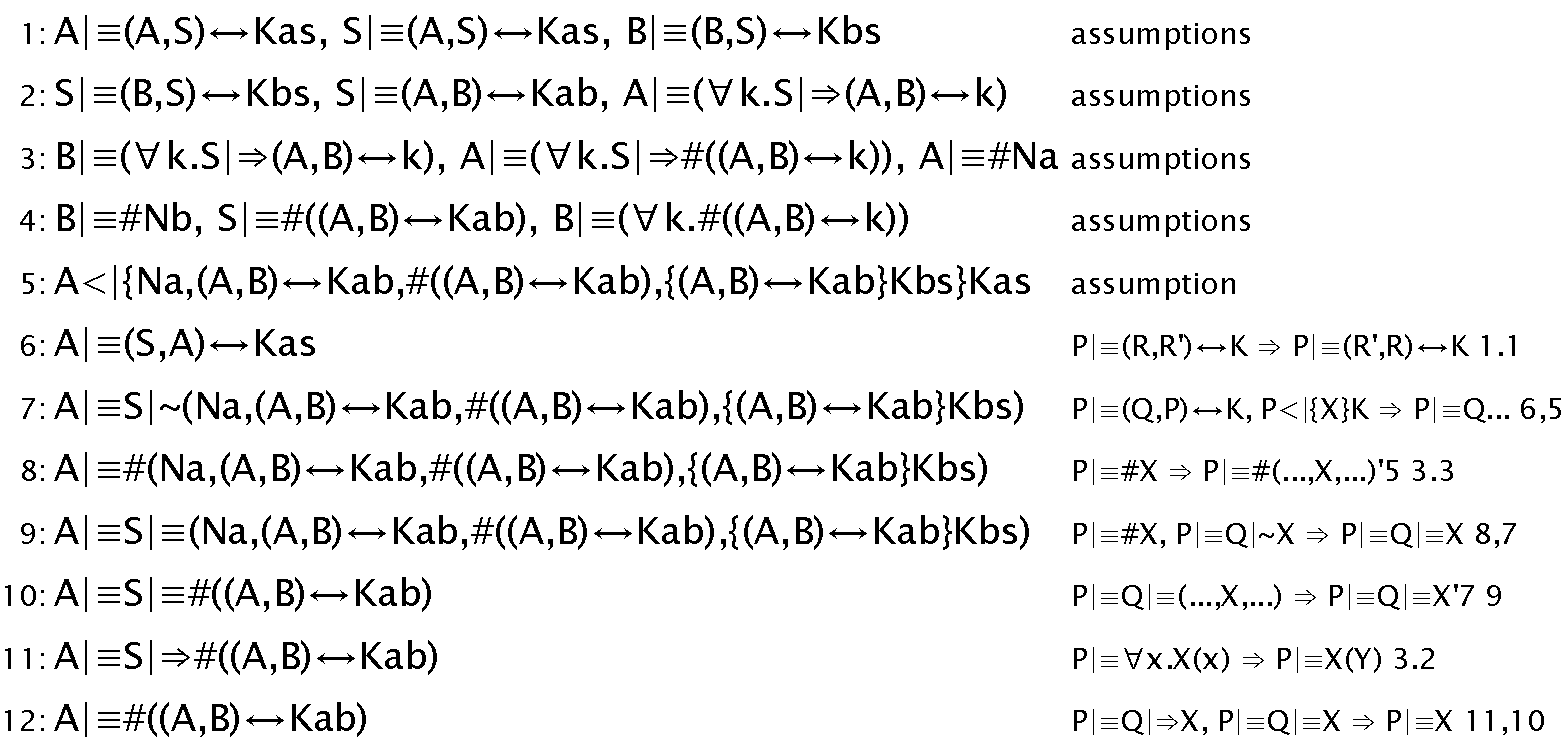
\includegraphics[scale=0.5]{pics/BAN/NSexample1}
\caption{A proof with a folded assumption line}
\label{fig:BAN:NSexample1}
\end{figure}

 